% Weekly update: support metrics, per-window mu and alpha, learned settings, and the current idea
% Compile: tectonic h2_weekly.tex
\documentclass[aspectratio=169,10pt]{beamer}
\usepackage[T1]{fontenc}
\usepackage{amsmath,amssymb,booktabs,graphicx,tabularx,xcolor,array}
\usepackage{tikz}
\usetikzlibrary{arrows.meta,positioning}
\graphicspath{{figures/}{/home/da25d400/arl_proj/rarl-proj/docs/h2_weekly/figures/}}

% Style of the HSM / HiPER weekly-meet deck: blue title bars, blue title box, plain footline
\usetheme{default}
\usefonttheme{professionalfonts}
\setbeamertemplate{navigation symbols}{}
\definecolor{bar}{HTML}{3333B3}
\definecolor{ok}{HTML}{1F6F43}
\definecolor{no}{HTML}{C0392B}
\setbeamercolor{structure}{fg=bar}
\setbeamercolor{frametitle}{fg=white,bg=bar}
\setbeamercolor{title}{fg=white,bg=bar}
\setbeamerfont{frametitle}{size=\Large}
\setbeamerfont{title}{size=\Large}
\setbeamertemplate{itemize items}[triangle]
\setbeamertemplate{enumerate items}[default]
\setbeamertemplate{frametitle}{%
  \nointerlineskip
  \begin{beamercolorbox}[wd=\paperwidth,ht=2.6ex,dp=1.4ex,leftskip=0.6em]{frametitle}
    \usebeamerfont{frametitle}\insertframetitle
  \end{beamercolorbox}\vspace{0.3em}}
\setbeamertemplate{title page}{%
  \vfill
  \begin{beamercolorbox}[wd=\textwidth,sep=10pt,center]{title}
    \usebeamerfont{title}\inserttitle\par\vspace{0.2em}
    \normalsize\insertsubtitle
  \end{beamercolorbox}\vspace{2em}
  \begin{center}
    \large\insertauthor\par\vspace{1em}
    \footnotesize\insertinstitute\par\vspace{1.2em}
    \large\insertdate
  \end{center}\vfill}
\setbeamertemplate{footline}{%
  \hspace{0.6em}\scriptsize\color{darkgray}\insertshorttitle\hfill
  \insertframenumber/\inserttotalframenumber\hspace{6em}\vspace{0.8em}}
\newcolumntype{Y}{>{\raggedright\arraybackslash}X}
\newcommand{\good}[1]{\textcolor{ok}{\textbf{#1}}}
\newcommand{\bad}[1]{\textcolor{no}{\textbf{#1}}}

\title[support metrics $\rightarrow$ per-window $\mu$ and $\alpha$ $\rightarrow$ current idea]{Does Every Window Need Its Own Editing Strength?}
\subtitle{Support metrics, support-based $\mu$ and $\alpha$, learned settings, and what we are trying now}
\author{Karan Kishore}
\institute{IIT Madras}
\date{Weekly Meet \,$|$\, October 28, 2026}

\begin{document}

\begin{frame}
\titlepage
\end{frame}

\begin{frame}{Roadmap}
\begin{enumerate}
\item \textbf{Setting}: the data, the score, and what GTA does to the data.
\item \textbf{Three ways to measure support} (how well-covered a window is), and why we trust them.
\item \textbf{Choosing the editing strength $\mu$ from support}: effect on the trained policy.
\item \textbf{Choosing the reward push $\alpha$}: why the score rises and then falls.
\item \textbf{Letting an optimiser (CMA-ES) choose $\mu$ and $\alpha$} for each window.
\item \textbf{What the support groups actually contain}, and why support did not help.
\item \textbf{Looking at the windows} in the simulator.
\item \textbf{The current idea}: repairing whole edited windows.
\end{enumerate}
\end{frame}

% =============================================================================================
\section{Setting}
\begin{frame}{The setting: learning from a fixed dataset}
\textbf{Offline reinforcement learning:} a policy is trained only from recorded data; it never interacts with the environment while learning.
\vspace{0.5em}

\textbf{Environment:} HalfCheetah, a simulated two-legged cheetah. The reward at each step is essentially its forward speed.
\vspace{0.3em}

\textbf{Dataset:} \texttt{halfcheetah-medium-v2}, 1{,}000 runs of 1{,}000 steps each, recorded by one medium-skill policy that runs at about 5 m/s.
At every step we have the \emph{state} (17 numbers: body angles and velocities), the \emph{action} (6 motor forces) and the reward.
\vspace{0.5em}

\textbf{Score:} we train TD3+BC (a standard offline RL algorithm) and run the trained policy. Its total reward is rescaled so that
\begin{center}
a random policy scores \textbf{0} \qquad and \qquad an expert policy (about 12 m/s) scores \textbf{100}.
\end{center}
Training on the dataset alone gives \textbf{48.7}.
\end{frame}

\begin{frame}{What GTA does: edit short windows to earn more reward}
\begin{columns}[T]
\begin{column}{0.48\linewidth}
A \textbf{window} is 31 consecutive steps of one run (states, actions, rewards) plus the final next state.
\vspace{0.4em}

GTA (Lee et al., NeurIPS 2024) trains a \emph{diffusion model} on all windows. A diffusion model learns to turn random noise back into realistic windows.
\vspace{0.4em}

To \textbf{edit} a window, GTA
\begin{enumerate}
\item adds a chosen amount of noise to it,
\item lets the model remove the noise while asking for a higher total reward,
\item adds the edited window to the training data.
\end{enumerate}
\end{column}
\begin{column}{0.5\linewidth}
Two settings control an edit:
\vspace{0.3em}

\textbf{$\mu$, editing strength (0 to 1):} how much noise is added, i.e.\ how much of the window is rewritten. Small $\mu$: a light touch-up. GTA uses $\mu = 0.5$.
\vspace{0.4em}

\textbf{$\alpha$, reward push:} the edit asks for $\alpha \times$ the window's original return. $\alpha = 1$: no push. GTA uses $\alpha = 1.3$.
\vspace{0.6em}

GTA uses the \textbf{same} $\mu$ and $\alpha$ for every window. With them, the score rises from 48.7 to about \textbf{58.5}.
\end{column}
\end{columns}
\end{frame}

\begin{frame}{The question}
\textbf{Hypothesis:} the best editing strength $\mu$ differs from window to window, and depends on two properties of the window:
\vspace{0.4em}
\begin{itemize}
\item \textbf{Support:} how many similar windows the dataset contains. Expectation: the model knows well-covered regions, so those windows can be edited \emph{more strongly} without becoming unrealistic.
\item \textbf{Quality:} how much reward the window itself earns. Expectation: a window that is already good has less to gain, so it should be edited \emph{less}.
\item \textbf{Downstream:} choosing $\mu$ per window should raise the TD3+BC score.
\end{itemize}
\vspace{0.5em}
To test this we need a number for the quality and a number for the support of every window.
\vspace{0.3em}

\textbf{Physics error}, used throughout: we replay an edited window in the real simulator and measure how far each step's claimed next state is from the state the simulator actually produces. An edit counts as \textbf{broken} when this error is larger than the average error reported in the GTA paper (0.0085).
\end{frame}

% =============================================================================================
\section{Metrics}
\begin{frame}{Quality: the reward a window earns}
\[
q_i = \sum_{t=0}^{30} 0.99^{\,t}\, r_{b_i+t}
\]
\begin{itemize}
\item $r_{b_i+t}$: the reward at step $t$ of window $i$, which starts at step $b_i$ of its run.
\item $0.99^{t}$ gives slightly less weight to later steps (the usual discount in RL).
\item Every metric is turned into a \textbf{percentile}: the fraction of all windows with a lower value. A window with quality percentile 0.9 earns more than 90\% of windows.
\end{itemize}
\vspace{0.5em}
\textbf{Typical values} (20{,}000 random windows): 10\% of windows earn less than 102, half earn less than 134, 90\% earn less than 152.
\vspace{0.5em}

\textbf{Why only the reward inside the window?} The reward still to come until the end of the run shrinks for windows late in a run even if the running is equally good, so it would describe \emph{position} in the run rather than behaviour.
\end{frame}

\begin{frame}{Support: three ways to measure how familiar a window is}
A window has \textbf{high support} when the dataset contains many similar situations (similar postures, speeds and motor forces), and \textbf{low support} when it is unusual, for example the first steps of a run when the cheetah speeds up from rest.
\vspace{0.6em}

Support cannot be observed directly, so we estimated it in three independent ways:
\vspace{0.4em}

\renewcommand{\arraystretch}{1.25}
\begin{tabularx}{\linewidth}{@{}lYl@{}}
\toprule
name & what it asks & cost\\
\midrule
$S_1$ & \textbf{the data:} how far away are the 20 most similar moments from other runs? & fast\\
$S_2$ & \textbf{the model:} how well can the diffusion model repair the window after we add noise? & fast\\
$S_3$ & \textbf{the model:} how probable does the model consider the window, computed exactly? & very slow\\
\bottomrule
\end{tabularx}
\vspace{0.6em}

$S_2$ is the one we used for all experiments. $S_1$ and $S_3$ are there to check it.
\end{frame}

\begin{frame}{$S_1$: distance to similar moments in other runs}
\begin{enumerate}
\item Put all 23 numbers of a step (17 state, 6 action) on a common scale: subtract each number's dataset average and divide by its spread (standard deviation). A difference of 1 then means ``one usual spread'' for every quantity.
\item For each of the 31 steps of the window, find the \textbf{20th most similar step} among the 1{,}000{,}000 steps of \emph{other} runs and record its distance:
\[
d = \sqrt{\textstyle\sum_{k=1}^{23} (z_k - z'_k)^2}\quad\text{(straight-line distance over the 23 numbers)}
\]
\item The window's value is the middle value (median) of these 31 distances.
\end{enumerate}
\vspace{0.3em}
\textbf{Reading it:} a short distance means many runs pass through similar situations (crowded region, high support); a long distance means the window is unusual.
\vspace{0.3em}

\textbf{Why other runs only:} neighbouring steps of the same run are nearly identical, so they would always be the closest and say nothing about coverage.
\vspace{0.3em}

\textbf{Typical values:} half of the windows have a distance below 1.10; 90\% are below 1.49; the most unusual reach 10.
\end{frame}

\begin{frame}{$S_2$: how well the model repairs a noisy window}
\begin{enumerate}
\item Take the window (all 32 rows $\times$ 24 numbers, on the common scale).
\item Add random noise of strength $\sigma$. We use three strengths, $\sigma = 0.16,\ 0.5,\ 2.4$: exactly the amounts of noise GTA adds when it edits with $\mu \approx 0.25,\ 0.35,\ 0.5$.
\item Ask the diffusion model to remove the noise in one step, without asking for any particular reward.
\item Measure the \textbf{repair error}: the average squared difference between the repaired window and the original, over all its numbers.
\item Repeat 4 times with fresh noise and average, so one lucky or unlucky draw does not decide.
\item Combine the three noise strengths: for each strength, compare the window's error with all other windows' errors; average the three comparisons. \textbf{Smaller error $\Rightarrow$ higher $S_2$.}
\end{enumerate}
\vspace{0.3em}
\textbf{Typical errors} (median window): 0.0045 at $\sigma = 0.16$, 0.022 at $\sigma = 0.5$, 0.15 at $\sigma = 2.4$.
\end{frame}

\begin{frame}[shrink=5]{Why the repair error measures support}
\textbf{Analogy.} Show a person a smudged photo of a common street sign: they read it correctly. Show them a smudged photo of a sign they have never seen: they guess, and usually guess wrong. How well someone can un-smudge a picture tells you how familiar that kind of picture is to them.
\vspace{0.6em}

\textbf{For the diffusion model:}
\begin{itemize}
\item It was trained to remove noise from the windows of this dataset.
\item For a kind of window it has seen many times, it removes the noise accurately: \textbf{small error, high support}.
\item For a rare kind of window, it ``repairs'' it towards the common windows it knows: \textbf{large error, low support}.
\end{itemize}
\vspace{0.6em}
\textbf{Link to probability:} it is a known property of diffusion models that windows the model considers more probable are repaired with smaller error. So $S_2$ is a cheap stand-in for ``how probable does the model find this window''. The exact version of that question is $S_3$ (next slide).
\vspace{0.4em}

\textbf{Why these three noise strengths:} they are the noise levels an actual edit uses, so $S_2$ asks ``can the model handle this window under the noise it will get when we edit it?''
\end{frame}

\begin{frame}{$S_3$: the exact probability the model gives a window}
\begin{itemize}
\item $S_3$ is the logarithm of the probability density the trained diffusion model assigns to the window: \textbf{higher means the model finds the window more likely}.
\item \textbf{How it is computed, in words:} the window is moved, smoothly and without any randomness, from its clean form to pure noise along a path fixed by the model. Where it ends up in the noise has a known probability. Along the way we keep track of how much the space around the window is stretched or squeezed. Combining ``where it ends up'' with ``how much it was stretched'' gives the window's exact probability under the model.
\item The stretching is tracked with a standard random shortcut (Hutchinson's trick) so it costs one extra network pass per step instead of 768.
\item It takes minutes per window, so we computed it for \textbf{100 random windows} only.
\end{itemize}
\vspace{0.4em}
\textbf{Values:} between 605 and 2{,}238 (log scale). The numbers are large because a window has 768 numbers and their contributions add up in the log; only the \emph{order} of windows matters.
\vspace{0.4em}

\textbf{Role:} $S_3$ is exactly what $S_2$ approximates, so it is the natural check for $S_2$. It is the model's view, not the absolute truth about the data.
\end{frame}

\begin{frame}[shrink=4]{The three support metrics side by side}
\renewcommand{\arraystretch}{1.35}
\begin{tabularx}{\linewidth}{@{}lYYY@{}}
\toprule
 & $S_1$ distance to similar moments & $S_2$ repair error & $S_3$ exact probability\\
\midrule
looks at & each step separately & the whole window & the whole window\\
uses the model & no & yes & yes\\
cost for 20{,}000 windows & seconds & about 3 seconds & only 100 windows feasible\\
main strength & direct, no model needed & tests the model at the noise editing uses & exact for the model\\
main weakness & ignores the order of steps; every number weighs equally & depends on the model; 3 noise levels chosen by hand & very slow; one random shortcut per window\\
role & cross-check & \textbf{used in all experiments} & check for $S_2$\\
\bottomrule
\end{tabularx}
\end{frame}

% =============================================================================================
\section{Validity}
\begin{frame}{How we check that the metrics mean something}
There is no ground truth for support, so we check three things:
\begin{enumerate}
\item \textbf{Agreement:} do the three metrics, built on different ideas, put windows in a similar order?
\item \textbf{Not just quality:} is support different from simply ``earns a lot of reward''?
\item \textbf{Prediction:} does support predict which edits break physics, as the hypothesis says it should?
\end{enumerate}
\vspace{0.5em}
\textbf{The tool: rank correlation} (Spearman's $\rho$). Sort the windows by metric A and by metric B, and compare the two orderings.
\begin{itemize}
\item $\rho = +1$: identical order. \quad $\rho = 0$: unrelated. \quad $\rho = -1$: exactly reversed.
\item Rough guide: around $\pm0.3$ a weak but real tendency; around $\pm0.8$ strongly related.
\item Only the order is compared, so it does not matter that the metrics have different units.
\end{itemize}
\vspace{0.3em}
Each $\rho$ comes with a 95\% range: we re-draw the windows at random 5{,}000 times, recompute $\rho$, and keep the middle 95\% of the results.
\end{frame}

\begin{frame}{Agreement: $S_2$ and $S_1$ against the exact probability $S_3$}
\centering
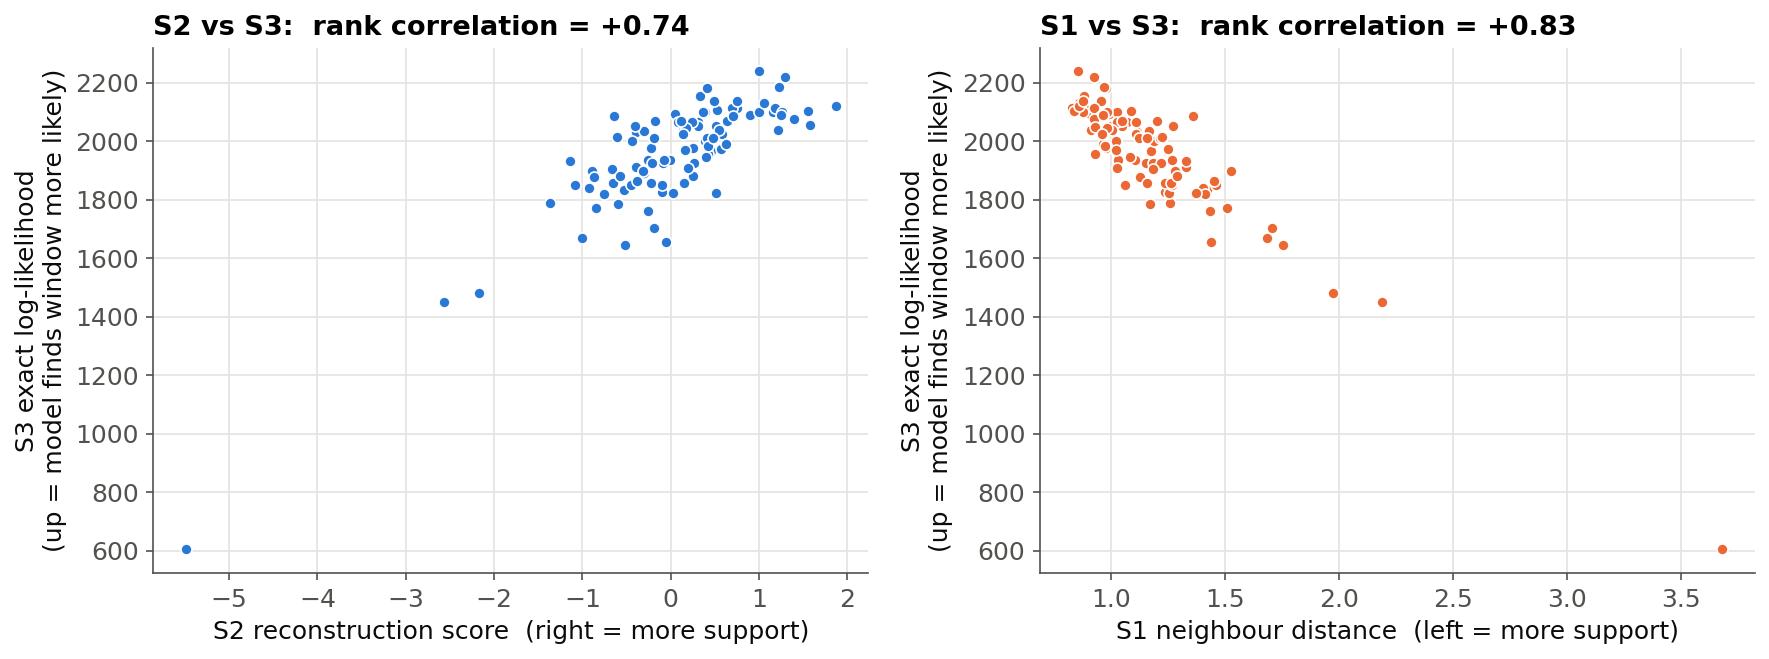
\includegraphics[width=0.76\linewidth]{s3_agree.png}

\raggedright\small
Each dot is one of the 100 windows for which $S_3$ was computed. \textbf{Vertical axis:} $S_3$, higher = the model finds the window more likely. \textbf{Left, horizontal:} the $S_2$ score, further right = smaller repair error. \textbf{Right, horizontal:} the $S_1$ distance, further left = more similar moments nearby.
\begin{itemize}
\item Left: dots rise from left to right, $\rho = 0.74$ (95\% range 0.62 to 0.82). Right: dots fall from left to right, $\rho = 0.83$.
\item The single window at the bottom (605 on $S_3$) is extreme on all three metrics; without it the correlations barely change (0.73 and 0.82).
\end{itemize}
\end{frame}

\begin{frame}{Is $S_2$ just noisy? Re-measuring it more carefully}
\textbf{Question:} $S_2$ uses only 4 random noise draws per strength. Is that why it is not closer to $S_3$?
\vspace{0.3em}

\textbf{Test:} recompute $S_2$ on the same 100 windows four more times, each with 4 fresh draws, and also with all 16 draws together.
\vspace{0.4em}

\centering
\begin{tabular}{lc}
\toprule
version of $S_2$ & rank correlation with $S_3$\\
\midrule
original (4 draws) & 0.74\\
four new sets of 4 draws & 0.76, 0.76, 0.76, 0.74\\
\textbf{16 draws} & \textbf{0.80} (95\% range 0.69 to 0.87)\\
\midrule
only the weakest noise, $\sigma = 0.16$ & 0.75\\
only the middle noise, $\sigma = 0.5$ & 0.71\\
only the strongest noise, $\sigma = 2.4$ & 0.66\\
\bottomrule
\end{tabular}
\vspace{0.5em}

\raggedright
\begin{itemize}
\item Two independent 4-draw versions order windows almost the same way ($\rho = 0.88$ with each other), so the randomness is small. More draws close only part of the gap (0.74 $\to$ 0.80).
\item The rest is by design: $S_2$ looks only at the noise levels editing uses, while the exact probability depends most on very fine detail (the weakest noise tracks $S_3$ best).
\end{itemize}
\end{frame}

\begin{frame}{Support is not quality, and it predicts broken edits}
\textbf{Not just quality:} rank correlation with quality is 0.42 for $S_2$ and 0.49 for $S_1$. Unusual windows tend to earn a bit less, but the two are far from the same, so they can be studied separately.
\vspace{0.6em}

\textbf{Prediction:} 400 windows were edited at 7 strengths and every edit was replayed in the simulator. Rank correlation between a window's metric and the physics error of its edit:
\vspace{0.3em}

\centering
\begin{tabular}{lrrrrrrr}
\toprule
editing strength $\mu$ & 0.1 & 0.2 & 0.3 & 0.35 & 0.4 & 0.45 & 0.5\\
\midrule
$S_2$ (support) & $-0.29$ & $-0.36$ & $-0.34$ & $-0.28$ & $-0.24$ & $-0.18$ & $-0.13$\\
$S_1$ (support) & $-0.25$ & $-0.34$ & $-0.32$ & $-0.26$ & $-0.28$ & $-0.25$ & $-0.15$\\
quality & $+0.07$ & $+0.01$ & $+0.01$ & $+0.09$ & $+0.04$ & $-0.14$ & $-0.07$\\
\bottomrule
\end{tabular}
\vspace{0.5em}

\raggedright
\begin{itemize}
\item Negative = the more support, the \emph{smaller} the physics error. Both support metrics show this at every $\mu$; quality does not.
\item The effect is moderate and \textbf{fades towards $\mu = 0.5$}: with that much noise the model rewrites almost the whole window, so the original window matters less.
\end{itemize}
\end{frame}

% =============================================================================================
\section{Mu by support}
\begin{frame}[shrink=9]{Choosing $\mu$ from support: the experiment}
\begin{itemize}
\item \textbf{Same windows everywhere:} 161{,}291 windows (about 5 million edited steps). Only the $\mu$ given to each window changes between versions.
\item Windows are split into \textbf{5 equal groups by $S_2$} (quintiles), from least to most support.
\item \textbf{Support-matched:} more support gets a stronger edit. \textbf{Reversed:} the same values in the opposite order. \textbf{Same for all:} one $\mu$ with the same average. The reversed version checks that any gain comes from the \emph{matching}, not just from mixing different $\mu$ values.
\end{itemize}
\vspace{0.3em}
\centering
\begin{tabular}{llcccccc}
\toprule
 & version & group 1 & group 2 & group 3 & group 4 & group 5 & average\\
 & & (least) & & & & (most) & \\
\midrule
gentle & same for all & 0.30 & 0.30 & 0.30 & 0.30 & 0.30 & 0.3\\
 & support-matched & 0.20 & 0.25 & 0.30 & 0.35 & 0.40 & 0.3\\
 & reversed & 0.40 & 0.35 & 0.30 & 0.25 & 0.20 & 0.3\\
\midrule
GTA-level & same for all & 0.50 & 0.50 & 0.50 & 0.50 & 0.50 & 0.5\\
 & support-matched & 0.30 & 0.40 & 0.50 & 0.60 & 0.70 & 0.5\\
 & reversed & 0.70 & 0.60 & 0.50 & 0.40 & 0.30 & 0.5\\
\bottomrule
\end{tabular}
\vspace{0.3em}

\raggedright\small The gentle support-matched values follow the measured ``safe $\mu$'' per group (the strongest edit before physics breaks: 0.20 for the least supported windows up to 0.34 for the most supported). TD3+BC: 1 million training steps, 3 random seeds per version.
\end{frame}

\begin{frame}[shrink=4]{Choosing $\mu$ from support: effect on the trained policy}
\centering
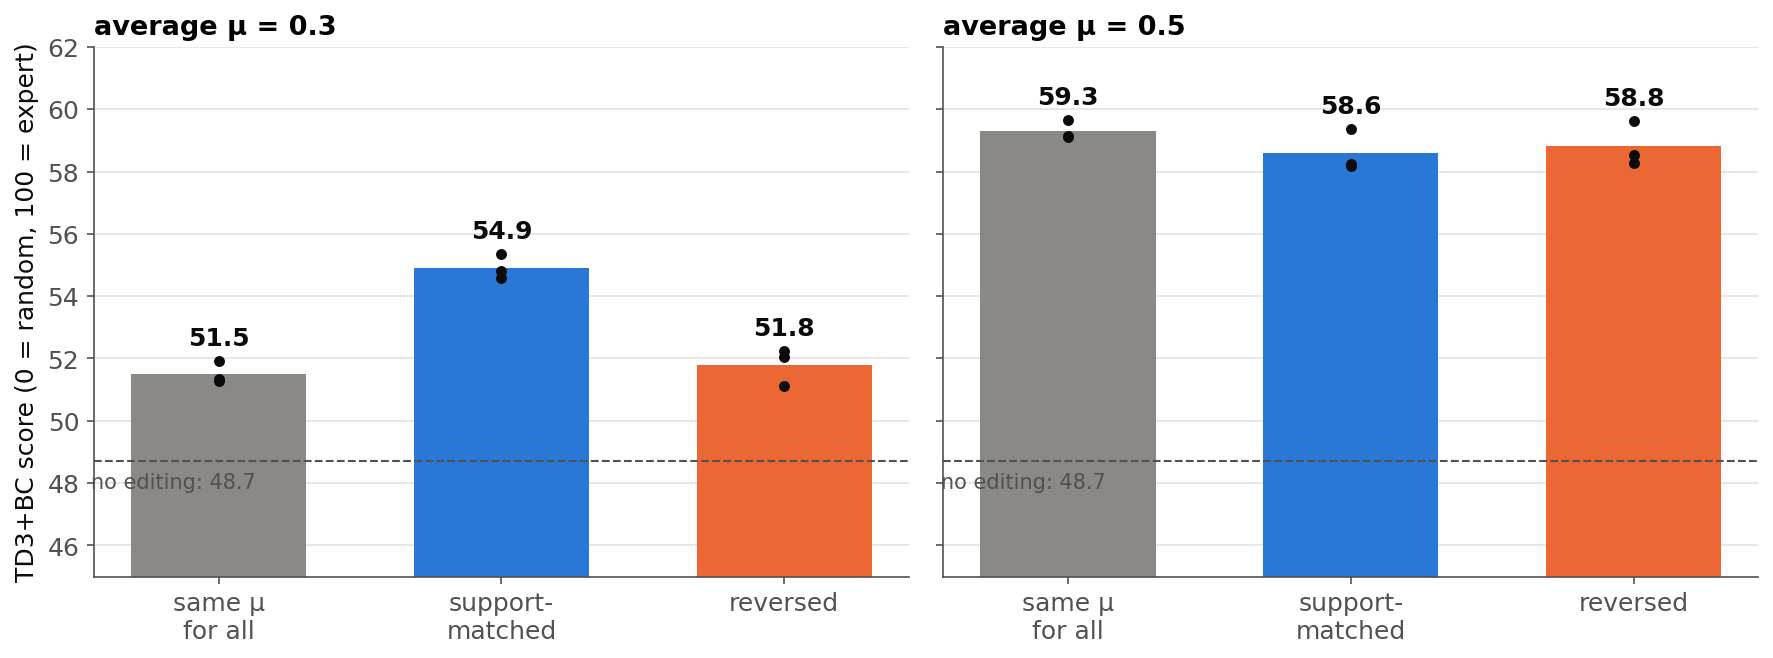
\includegraphics[width=0.7\linewidth]{mu_support_rl.png}

\raggedright\small
\textbf{Vertical axis:} TD3+BC score. \textbf{Bars:} average over 3 seeds; \textbf{black dots:} the individual seeds. \textbf{Dashed line:} training without any edited data (48.7).
\begin{itemize}
\item \textbf{Gentle editing (left):} support-matched beats same-for-all by \textbf{+3.4} and reversed by \textbf{+3.1}. The seeds do not overlap, and the result repeated in a second, independent implementation (+2.5 and +1.8).
\item \textbf{GTA-level editing (right):} support-matched is \textbf{not} better ($-0.7$ against same-for-all, within seed noise).
\item The best version overall is simply $\mu = 0.5$ for everyone (59.3). Support-based $\mu$ helps only in the gentle regime, which scores lower anyway.
\end{itemize}
\end{frame}

% =============================================================================================
\section{Alpha}
\begin{frame}{Choosing the reward push $\alpha$: the experiment}
$\mu$ is fixed at GTA's 0.5 and the reward push $\alpha$ is varied. 32{,}258 windows (1 million edited steps), TD3+BC as before.
\vspace{0.5em}
\begin{enumerate}
\item \textbf{One $\alpha$ for everyone:} 1.0, 1.1, 1.3, 1.5, 1.8, 2.0.
\item \textbf{$\alpha$ from support}, around the best value 1.3, using the same 5 support groups:
\begin{center}
\begin{tabular}{lccccc}
\toprule
version & group 1 (least) & group 2 & group 3 & group 4 & group 5 (most)\\
\midrule
up & 1.1 & 1.2 & 1.3 & 1.4 & 1.5\\
down & 1.5 & 1.4 & 1.3 & 1.2 & 1.1\\
random & \multicolumn{5}{c}{each window gets one of 1.1--1.5 at random}\\
\bottomrule
\end{tabular}
\end{center}
\end{enumerate}
\vspace{0.4em}
\textbf{How to read the second part:} if ``up'' beats ``random'', matching $\alpha$ to support matters. If ``up'' and ``random'' do equally well, only the \emph{mixing} of several $\alpha$ values matters.
\end{frame}

\begin{frame}{More reward push helps, up to a point}
\centering
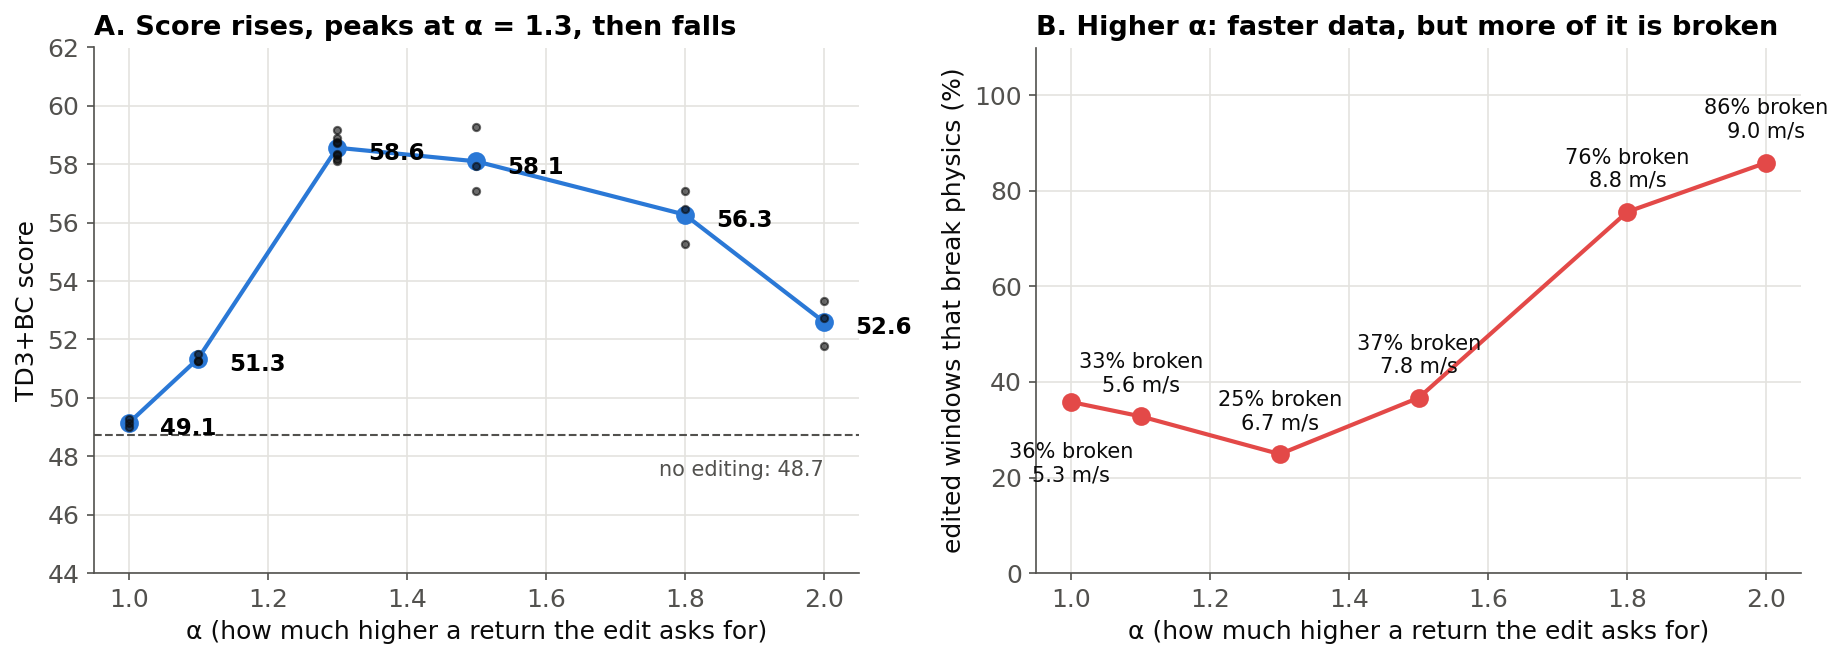
\includegraphics[width=0.8\linewidth]{alpha_curve.png}

\raggedright\small
\textbf{A:} horizontal = $\alpha$; vertical = TD3+BC score; big dots = average, small dots = seeds; dashed = no edited data.
\textbf{B:} same horizontal axis; vertical = share of edited windows whose physics error is above the paper's average; labels also give the edited data's average speed.
\begin{itemize}
\item From $\alpha = 1$ to 1.3 the edited data gets faster (5.3 $\to$ 6.7 m/s) while staying about as realistic, and the score climbs from 49.1 to \textbf{58.6}.
\item Beyond 1.3 the data keeps getting faster (up to 9 m/s), but the share of broken windows jumps (37\% $\to$ 76\% $\to$ 86\%) and the score falls to 52.6.
\end{itemize}
\end{frame}

\begin{frame}{Why the score falls: fast but impossible motions}
\begin{itemize}
\item \textbf{Reward is speed}, so faster edited data shows the policy how to earn more. The dataset itself never runs faster than about 7.3 m/s; GTA's edits at $\alpha = 1.3$ add running that is faster than almost anything in the data.
\item \textbf{But the model has never seen very fast running.} Asked for much more reward ($\alpha = 1.8$--2), it produces windows that look fast but cannot happen physically: in one rendered example the cheetah stands almost vertically on its back legs while supposedly moving at 10 m/s.
\item \textbf{TD3+BC learns from every step it is given.} Impossible steps teach it that certain actions lead to fast, high-reward states that the real simulator never reaches. The policy chases those, and the real score drops.
\end{itemize}
\vspace{0.5em}
\textbf{The trade-off in one line:} more speed in the data helps; broken physics hurts. $\alpha = 1.3$ is where the two balance.
\end{frame}

\begin{frame}[shrink=8]{Choosing $\alpha$ from support: results}
\centering
\begin{tabular}{lccc}
\toprule
version & score (mean $\pm$ spread) & seeds & compared with $\alpha = 1.3$ for all\\
\midrule
$\alpha = 1.3$ for all & 58.57 $\pm$ 0.38 & 8 & --\\
up (more push for more support) & 59.53 $\pm$ 0.51 & 8 & +0.96\\
down (less push for more support) & 59.18 $\pm$ 0.62 & 8 & +0.61\\
\midrule
\multicolumn{4}{l}{\emph{repeated with 5 new seeds, including the random control}}\\
$\alpha = 1.3$ for all & 58.66 $\pm$ 0.44 & 5 & --\\
up & 59.52 $\pm$ 0.58 & 5 & +0.87\\
down & 59.40 $\pm$ 0.58 & 5 & +0.74\\
random & 58.69 $\pm$ 1.72 & 5 & +0.04\\
\bottomrule
\end{tabular}
\vspace{0.6em}

\raggedright
\begin{itemize}
\item ``Up'' is reliably about +0.9 above a single $\alpha$, on both sets of seeds.
\item But ``down'' (the opposite direction) does nearly as well, and ``up'' cannot be told apart from ``random'' (the random version varies a lot between seeds).
\item \textbf{Conclusion:} mixing $\alpha$ values may help slightly; \textbf{matching $\alpha$ to support does not clearly matter}.
\end{itemize}
\end{frame}

% =============================================================================================
\section{Learned settings}
\begin{frame}{Letting an optimiser choose $\mu$ and $\alpha$ per window}
Instead of hand-made rules, write $\mu$ and $\alpha$ as \textbf{smooth curves} of a window's support $S$ and quality $Q$ (both percentiles, shifted to run from $-0.5$ to $+0.5$):
\[
\mu_i = 0.3 + 0.4\cdot \operatorname{sig}(a_0 + a_S S_i + a_Q Q_i), \qquad
\alpha_i = 1.0 + 0.8\cdot \operatorname{sig}(c_0 + c_S S_i + c_Q Q_i)
\]
\begin{itemize}
\item $\operatorname{sig}(z) = 1/(1+e^{-z})$ squeezes any number into the range 0 to 1, so $\mu$ always stays between 0.3 and 0.7 and $\alpha$ between 1.0 and 1.8.
\item The six numbers $a_0, a_S, a_Q, c_0, c_S, c_Q$ decide the rule. Example: $a_S > 0$ means more support gets a stronger edit; $a_S = a_Q = c_S = c_Q = 0$ means one $\mu$ and one $\alpha$ for everyone.
\end{itemize}
\vspace{0.4em}
\textbf{Goal:} find the six numbers that give the highest TD3+BC score.
\vspace{0.3em}

\textbf{Difficulty:} the score is only known after generating edited data and training a policy (minutes per try), and there is no formula telling us which direction improves it. We need a search method that only needs ``try a setting, observe its score''. We used \textbf{CMA-ES}.
\end{frame}

\begin{frame}[shrink=4]{CMA-ES explained: guided trial and error}
\centering
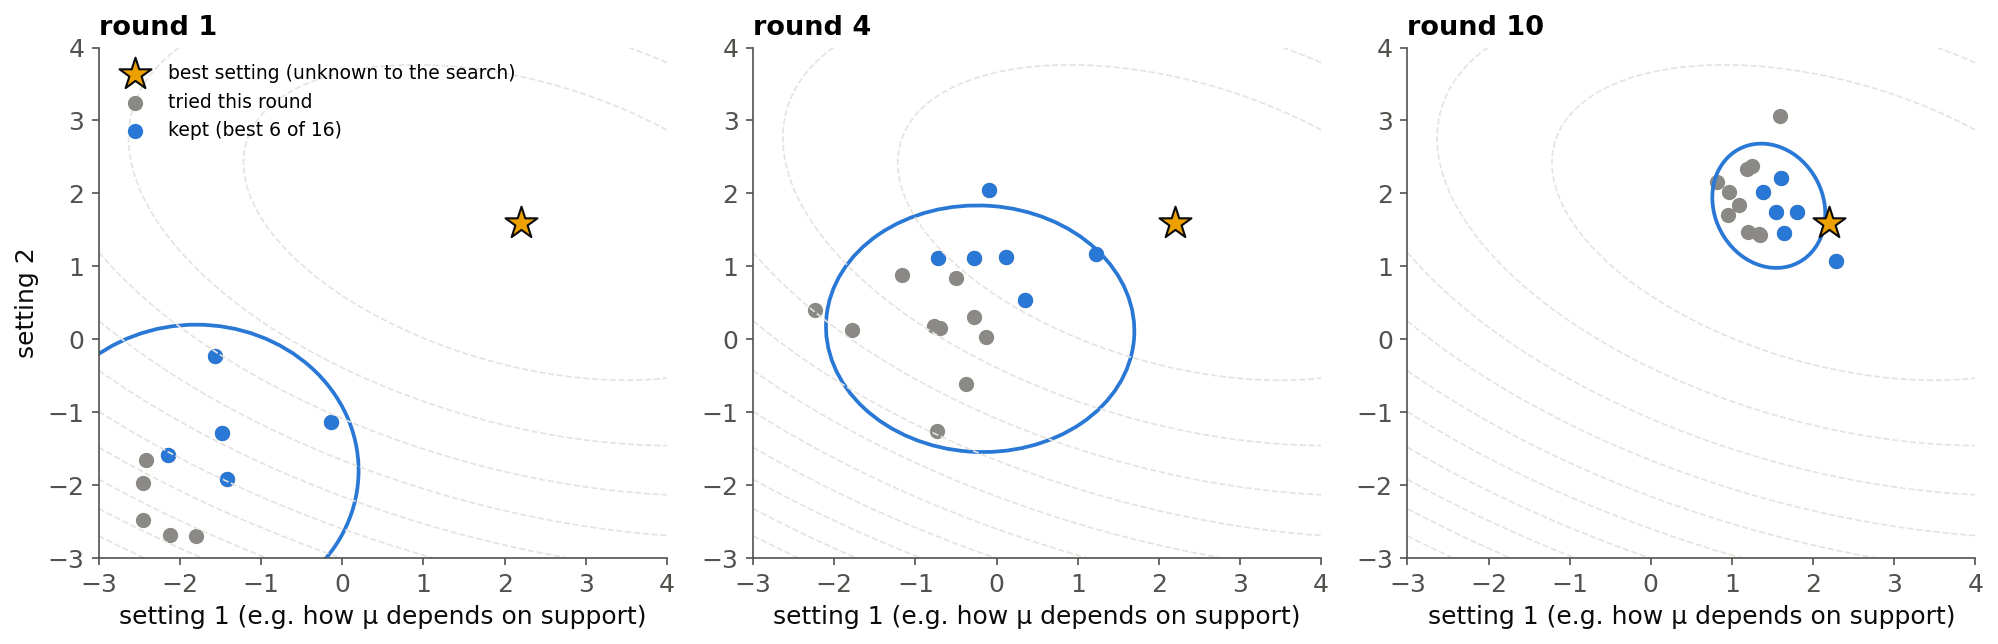
\includegraphics[width=0.74\linewidth]{cmaes_toy.png}

\raggedright\small
A toy problem with two settings (horizontal and vertical axes). Grey contour lines mark equal score; the star is the best setting, which the search does not know. Each round:
\begin{enumerate}
\item \textbf{Try:} draw 16 settings at random from a cloud (the blue ellipse marks where the cloud is). Measure each one's score.
\item \textbf{Keep the best:} take the best 6 (blue dots); drop the rest (grey).
\item \textbf{Move and reshape the cloud:} new centre = average of the kept settings. The cloud is stretched along the direction in which the kept settings lie and in which the centre just moved, and shrinks when progress slows.
\end{enumerate}
Round 1: the cloud is far away. Round 4: it has moved towards better scores. Round 10: it has shrunk around the star.
\end{frame}

\begin{frame}{CMA-ES in a little more detail}
\textbf{The name:} Covariance Matrix Adaptation Evolution Strategy.
\begin{itemize}
\item \textbf{Evolution strategy:} like breeding. Each round produces a ``population'' of candidate settings; the fittest survive and the next population is drawn around them.
\item \textbf{Covariance matrix:} the shape of the cloud (how wide it is in each direction, and how tilted). ``Adaptation'' means this shape is learned from which candidates did well.
\end{itemize}
\vspace{0.4em}
\textbf{What one round does, precisely:}
\begin{enumerate}
\item Draw candidates $x_k = m + s \cdot (\text{random step shaped by the cloud})$, where $m$ is the centre and $s$ the overall step size.
\item Score each $x_k$ (here: generate data, train TD3+BC, read the score).
\item New centre $m$ = weighted average of the best candidates (better ones count more).
\item Update the cloud shape towards the directions of the successful steps, and remember the recent direction of travel so consistent progress stretches the cloud further.
\item Make $s$ larger if the centre keeps moving in the same direction (far from the goal), smaller if it jumps back and forth (close to the goal).
\end{enumerate}
\vspace{0.3em}
\textbf{Why it suits us:} it needs only scores, tolerates noisy scores, and works well with a handful of settings (here 6).
\end{frame}

\begin{frame}{The search, and what it learned}
\centering
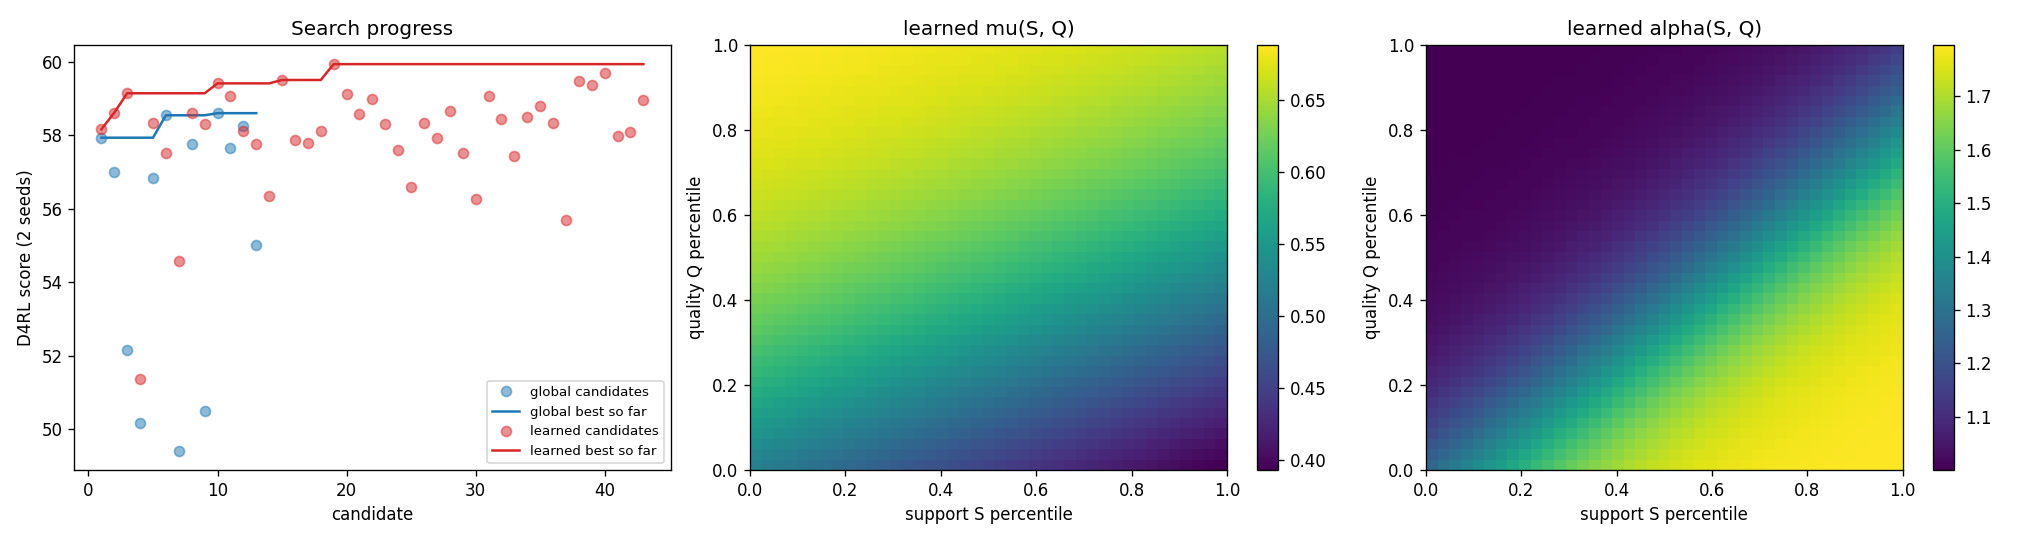
\includegraphics[width=\linewidth]{search.png}

\raggedright\small
\textbf{Left:} horizontal = candidate number in the order tried; vertical = score (2 seeds, half-size data). Blue = searching one $\mu$ and one $\alpha$ for everyone (13 tries); red = searching the full per-window rule (43 tries); lines = best so far.
\textbf{Middle / right:} the best per-window rule found. Horizontal = support percentile, vertical = quality percentile, colour = $\mu$ (middle) and $\alpha$ (right) that the rule gives such a window.
\begin{itemize}
\item The learned rule gives \emph{lower} $\mu$ to well-supported windows and pushes $\alpha$ hard only for well-supported, low-quality windows: the opposite of our hypothesis for $\mu$.
\end{itemize}
\end{frame}

\begin{frame}{Confirming the winners on fresh seeds}
\begin{columns}[T]
\begin{column}{0.45\linewidth}
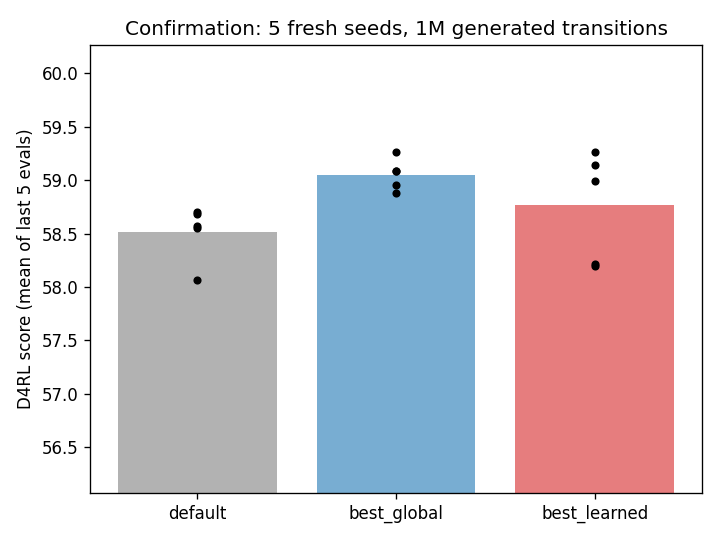
\includegraphics[width=\linewidth]{confirm_bars.png}

\scriptsize Vertical = score (note: the axis starts at 56); bars = average of 5 new seeds; dots = individual seeds.
\end{column}
\begin{column}{0.53\linewidth}
\small
\begin{tabular}{@{}lccc@{}}
\toprule
setting & score & avg.\ $\mu$ & avg.\ $\alpha$\\
\midrule
GTA default & 58.51 & 0.500 & 1.300\\
best single $\mu$, $\alpha$ & \textbf{59.05} & 0.565 & 1.356\\
best per-window rule & 58.76 & 0.592 & 1.277\\
\bottomrule
\end{tabular}
\vspace{0.5em}
\begin{itemize}
\item The per-window rule is \textbf{not} better than one well-chosen $\mu$ and $\alpha$ ($-0.29$, within seed noise).
\item During the search it looked better (59.9), but that came from luck: when 43 settings are each tried on only 2 seeds, one of them looks good by chance.
\item A slightly stronger single setting (0.565, 1.356) gives a small real gain over GTA's default: +0.54.
\end{itemize}
\end{column}
\end{columns}
\end{frame}

% =============================================================================================
\section{Why support did not help}
\begin{frame}{What the support groups actually contain}
\centering
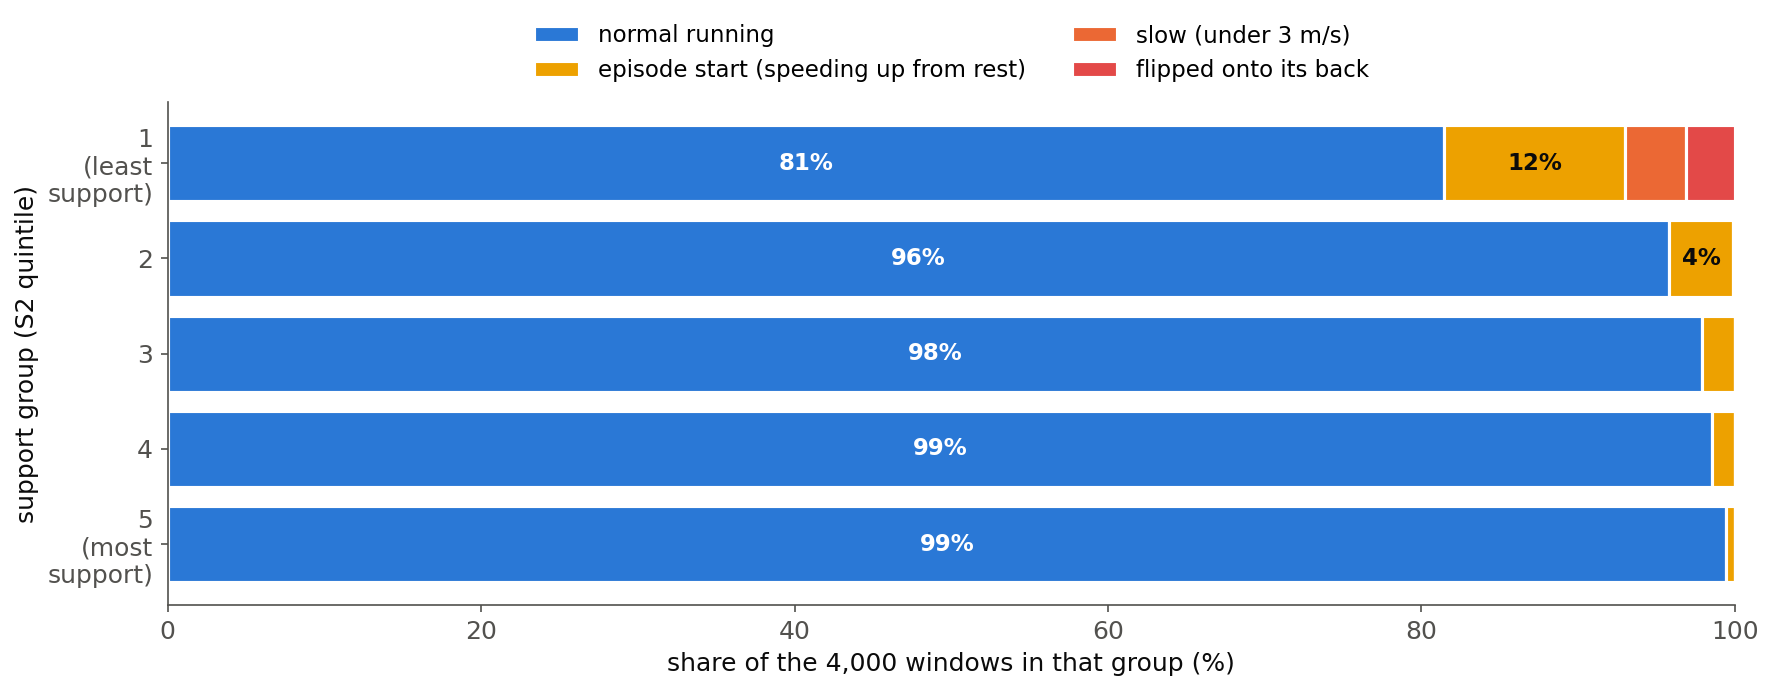
\includegraphics[width=0.85\linewidth]{quintile_content.png}

\raggedright\small
20{,}000 windows, split into 5 equal groups by $S_2$ (rows, least support at the top). Each bar shows what kinds of windows the group contains; horizontal axis = share of the group. Categories come from the cheetah's body angle, speed and position in its run.
\begin{itemize}
\item Even the least-supported group is \textbf{81\% normal running}. The truly unusual windows (flips, slow-downs, starts from rest) are only about 5\% of all data, and they all sit in group 1.
\item Groups 2 to 5 are 96--99\% normal running and differ only in small details.
\end{itemize}
\end{frame}

\begin{frame}{Why support-based $\mu$ and $\alpha$ could not do much here}
\begin{itemize}
\item \textbf{One policy, one way of running.} The dataset was recorded by a single medium-skill policy, so about 95\% of all windows are the same kind of steady running. Support differences between most windows are small.
\item \textbf{The unusual windows are few and not useful to edit.} A cheetah lying on its back gains nothing from a stronger or weaker edit; these windows are a small part of the data either way.
\item \textbf{At GTA's own setting the original window matters little.} With $\mu = 0.5$ the model rewrites most of the window, so how familiar the original was hardly changes the result (the link between support and physics error fades towards $\mu = 0.5$).
\item \textbf{Support describes the input, but RL is affected by the output.} Whether an edited window is realistic is a property of the edited window; the original's support predicts it only weakly.
\end{itemize}
\vspace{0.5em}
\textbf{Summary:} the support metric works (it finds the unusual windows), but on this dataset there is too little variation in support among the windows that matter for it to steer $\mu$ or $\alpha$ usefully.
\end{frame}

% =============================================================================================
\section{Visual check}
\begin{frame}{What low, medium and high support look like}
\centering
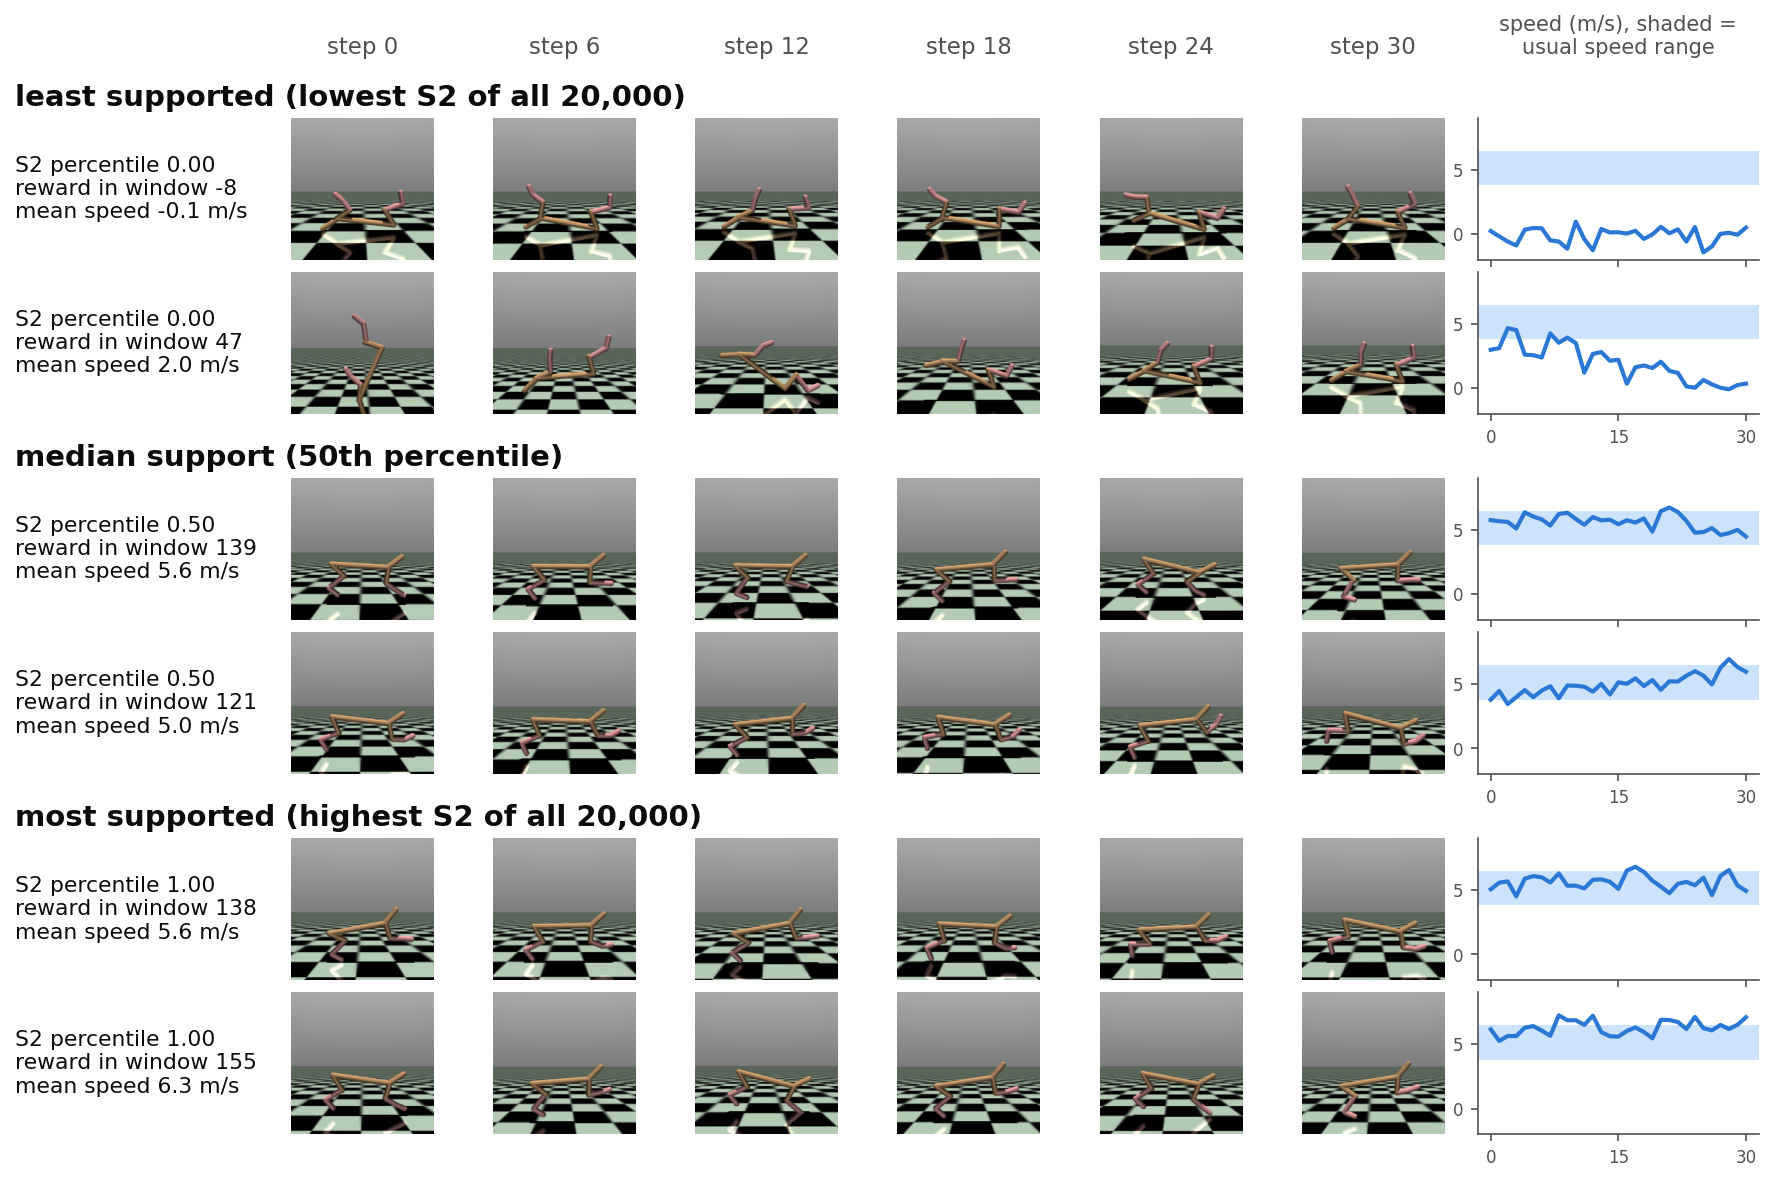
\includegraphics[height=0.78\textheight]{support_levels_slide.png}

\raggedright\scriptsize Two windows at each level, rendered in the simulator at 6 moments of the 31 steps. Right: forward speed over the window (blue line) and the dataset's usual speed range (shaded).
\end{frame}

\begin{frame}{Reading the renders}
\begin{itemize}
\item \textbf{Least supported:} the cheetah has \textbf{flipped onto its back} with its legs in the air (first window), or is rolling over (second window, upright at step 0, on its back by step 12). Speed falls to about 0, far below the usual range, and the window earns almost no reward.
\item \textbf{Median support:} normal running; speed stays inside the usual range with small ups and downs.
\item \textbf{Most supported:} the cleanest, most regular stride; the torso stays level and the legs repeat the same cycle every few steps.
\end{itemize}
\vspace{0.6em}
In numbers, over 20{,}000 windows:
\begin{itemize}
\item 94.6\% normal running, 4.0\% starts from rest, 0.8\% slow, 0.6\% flipped.
\item \textbf{All} 124 flipped windows, 97\% of the slow windows and 59\% of the starts fall in the least-supported fifth.
\end{itemize}
\vspace{0.4em}
So $S_2$ does what it should: it ranks stumbles and flips as unusual and steady running as familiar. The middle of the ranking separates only slightly irregular from slightly more regular running.
\end{frame}

\begin{frame}{Editing an unusual window with increasing $\mu$}
\begin{columns}[T]
\begin{column}{0.6\linewidth}
\centering
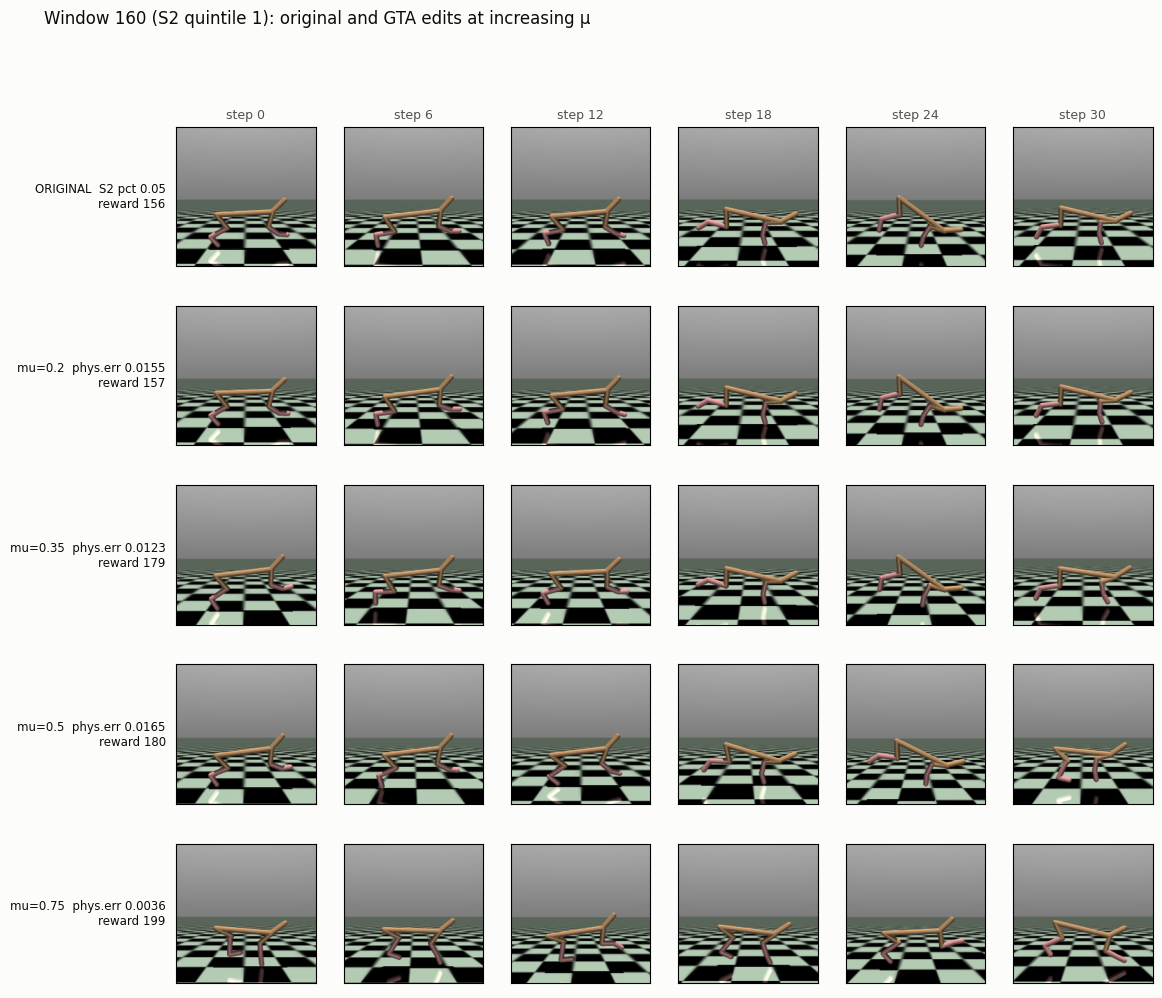
\includegraphics[width=\linewidth,height=0.83\textheight,keepaspectratio]{window160_edits.png}
\end{column}
\begin{column}{0.38\linewidth}
\footnotesize
A stumbling window (least-supported fifth): the body pitches nose-down at steps 18--24 and speed drops.
\vspace{0.3em}

Rows: the original, then GTA edits with $\mu = 0.2, 0.35, 0.5, 0.75$; columns: 6 moments of the window. Left labels: physics error and true reward.
\vspace{0.3em}
\begin{itemize}
\item $\mu = 0.2$--$0.5$: the edit keeps the stumble but pushes it towards more reward (156 $\to$ 180). Physics error is high (0.012--0.017, above the 0.0085 limit): the model forces an unusual motion it does not know well.
\item $\mu = 0.75$: the stumble disappears; the model replaces it with a normal stride (error 0.0036, reward 199). It is no longer the original window.
\end{itemize}
\end{column}
\end{columns}
\end{frame}

\begin{frame}{Editing a familiar window with increasing $\mu$}
\begin{columns}[T]
\begin{column}{0.6\linewidth}
\centering
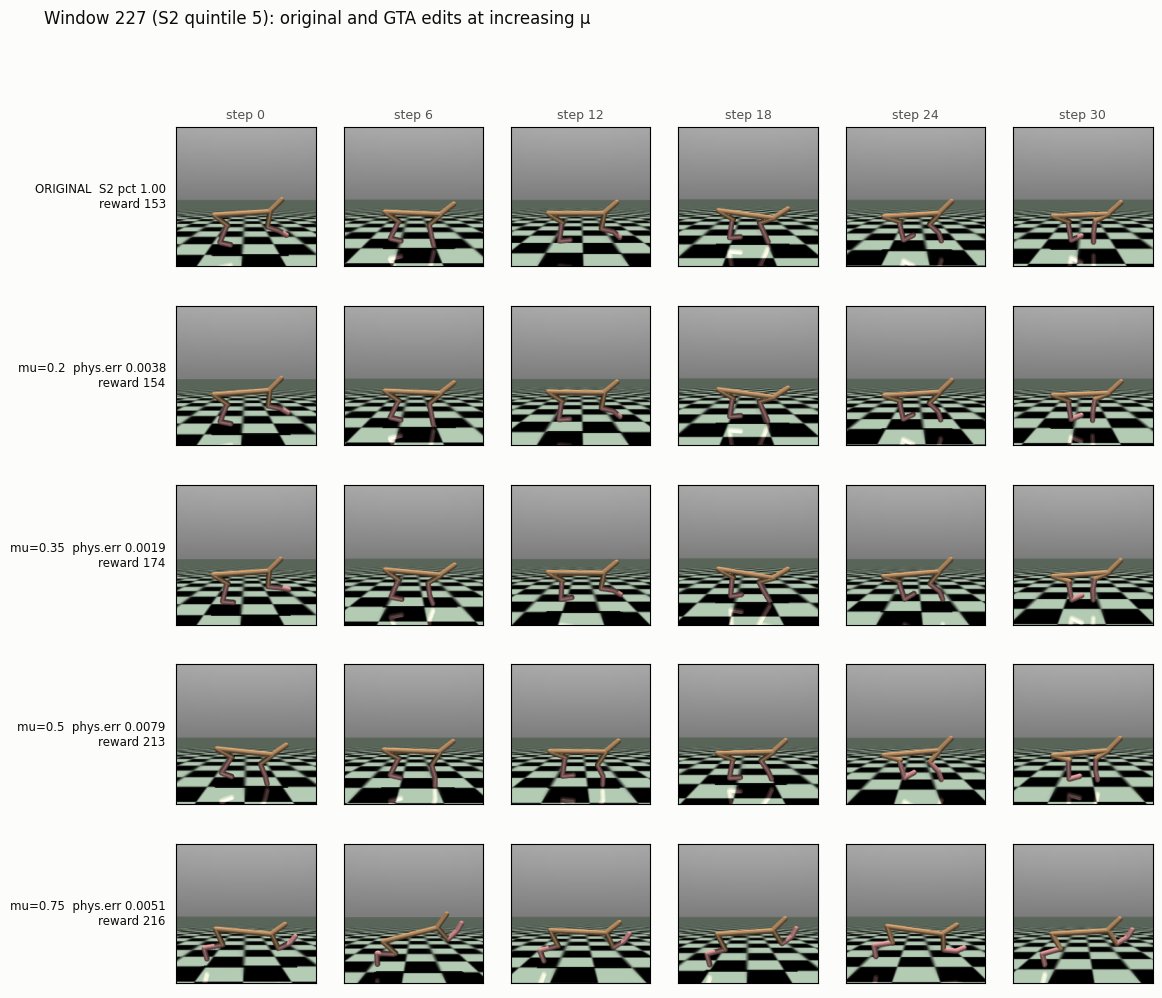
\includegraphics[width=\linewidth,height=0.83\textheight,keepaspectratio]{window227_edits.png}
\end{column}
\begin{column}{0.38\linewidth}
\footnotesize
A steady running window (most-supported fifth), same layout as before.
\vspace{0.3em}
\begin{itemize}
\item $\mu = 0.2$--$0.35$: almost the same motion, a bit faster (reward 153 $\to$ 174) with very low physics error (0.002--0.004).
\item $\mu = 0.5$: reward jumps to 213 (+39\%) while the error (0.0079) stays below the limit.
\item $\mu = 0.75$: the posture visibly changes into a longer, stretched stride.
\end{itemize}
\vspace{0.4em}
\textbf{Together with the previous slide:} familiar motions can be edited much more strongly before physics breaks; unusual ones break even under light edits. This is the support effect we measured, now visible. It is real, but it concerns few windows on this dataset.
\end{column}
\end{columns}
\end{frame}

% =============================================================================================
\section{Current idea}
\begin{frame}{What limits the score}
\centering
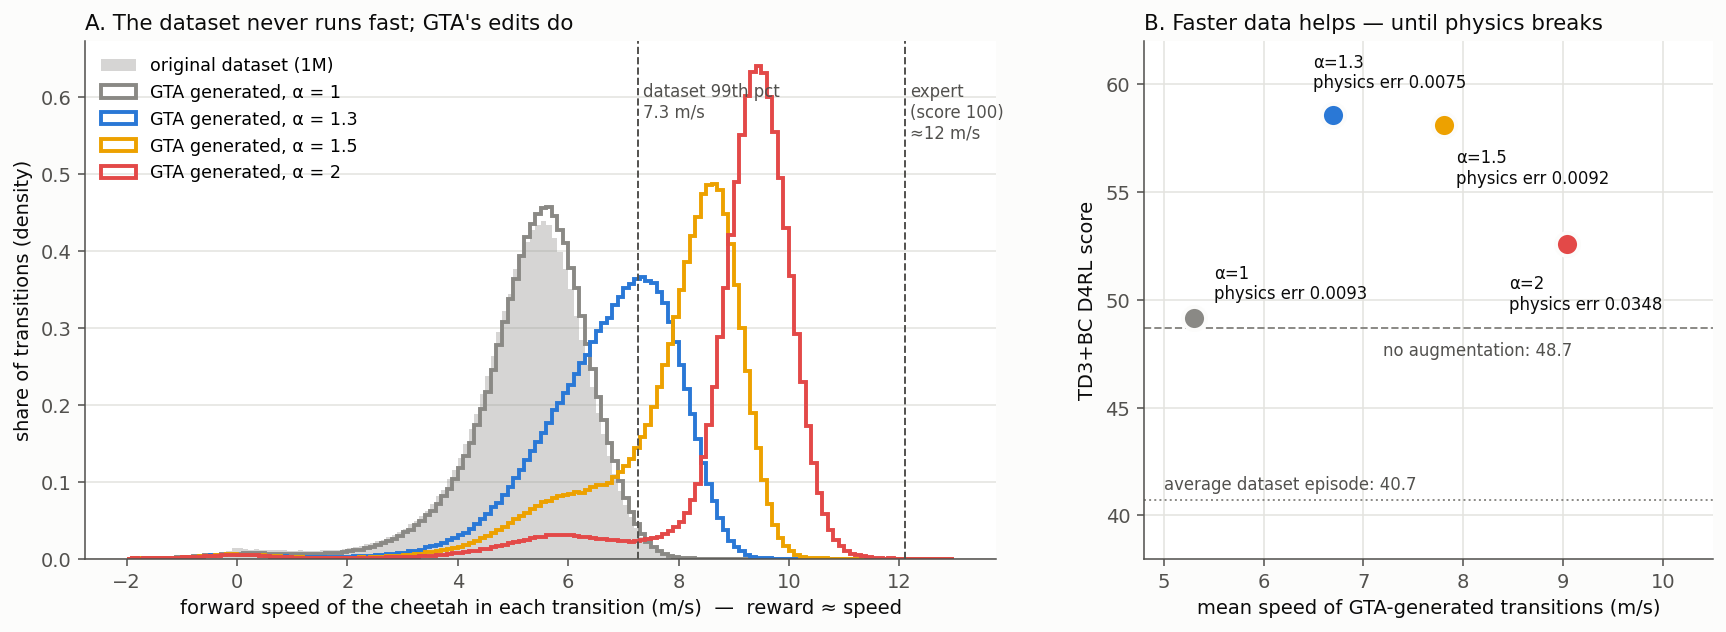
\includegraphics[width=0.82\linewidth]{why_gta.png}

\raggedright\small
\textbf{A:} horizontal = forward speed of each step; vertical = how common that speed is. Grey = the dataset; coloured lines = GTA's edited data for different $\alpha$. Dashed lines: the dataset's top 1\% speed (7.3 m/s) and the expert's speed (12 m/s).
\textbf{B:} horizontal = average speed of the edited data; vertical = TD3+BC score; labels give the data's physics error.
\begin{itemize}
\item The policy can only learn speeds the data shows. GTA helps by adding faster running; the limit is that \textbf{faster edits break physics}.
\end{itemize}
\end{frame}

\begin{frame}{What every attempt so far got right, and wrong}
For TD3+BC, edited data has to be three things \textbf{at the same time}:
\begin{enumerate}
\item \textbf{fast:} new, faster running than the dataset has;
\item \textbf{realistic:} each step follows the real physics;
\item \textbf{connected:} each step's next state is exactly the next step's starting state, so the 31 steps form one continuous motion. TD3+BC learns how valuable a state is by passing value backwards along these links (value here = reward now + value of where I end up).
\end{enumerate}
\vspace{0.4em}
\centering
\begin{tabular}{lccc}
\toprule
approach & fast & realistic & connected\\
\midrule
GTA with strong push ($\alpha = 1.8$--2) & \good{yes} & \bad{no} & \good{yes}\\
correct each step separately with a physics model & \good{yes} & \good{yes} & \bad{no}\\
re-simulate the whole window with a physics model & \bad{no} & \bad{no} & \good{yes}\\
\textbf{whole-window adjustment (current idea)} & \good{yes} & \good{yes} & \good{yes}\\
\bottomrule
\end{tabular}
\vspace{0.4em}

\raggedright\small Correcting each step separately made the data more realistic but lowered the score by about 2 points: the broken links stopped value from flowing back along the fast running.
\end{frame}

\begin{frame}{The current idea: adjust the whole window at once}
\textbf{Tool:} a small \emph{physics model} trained on the dataset only. Given a state and an action, it predicts the next state. It is accurate for \textbf{one} step but its small errors pile up over many steps. It is really 5 small networks; where they disagree, the model is unsure.
\vspace{0.5em}

\textbf{Method:} treat GTA's edited window as a draft and nudge \emph{every} state and \emph{every} action a little, all together, to satisfy three wishes at once:
\begin{enumerate}
\item \textbf{stay close to GTA's draft}, so its faster motion is kept;
\item \textbf{every single step obeys the physics model}: predicted next state $\approx$ the window's next state (only one-step predictions, where the model is accurate);
\item \textbf{stay where the 5 networks agree}, so the adjustment cannot exploit places where the model is wrong.
\end{enumerate}
\[
\text{minimise}\;\; \underbrace{\lVert \hat s - s_{\text{GTA}}\rVert^2}_{\text{close to draft}} + 0.1\,\underbrace{\lVert \hat a - a_{\text{GTA}}\rVert^2}_{\text{similar actions}} + 100\underbrace{\textstyle\sum_t \lVert \hat s_{t+1} - f(\hat s_t,\hat a_t)\rVert^2}_{\text{each step obeys physics}} + 10\cdot\underbrace{\text{disagreement}}_{\text{model is sure}}
\]
\small Repeated 500 times: ``move every state and action slightly in the direction that lowers this sum''. Each adjusted state is both the end of one step and the start of the next, so the window \textbf{stays connected automatically}.
\end{frame}

\begin{frame}{Why we expect it to help, and first checks}
\textbf{Reasoning:} the score is limited by how much \emph{fast and valid} running TD3+BC sees; strong pushes failed because their data broke physics; fixing physics step by step failed because it broke the links. The adjusted data is fast, realistic and connected.
\vspace{0.4em}

\textbf{First check, before any RL} (300 windows each, replayed in the real simulator):
\vspace{0.2em}

\centering
\begin{tabular}{lccc}
\toprule
data & speed & physics error & broken windows\\
\midrule
GTA default ($\alpha = 1.3$) & 6.7 m/s & 0.0075 & 25\%\\
GTA, $\alpha = 1.5$, as generated & 7.9 m/s & 0.0093 & 36\%\\
GTA, $\alpha = 1.5$, \textbf{adjusted} & \textbf{7.8 m/s} & \textbf{0.0049} & \textbf{6\%}\\
GTA, $\alpha = 1.8$, as generated & 8.8 m/s & 0.0190 & 77\%\\
GTA, $\alpha = 1.8$, \textbf{adjusted} & \textbf{8.7 m/s} & \textbf{0.0071} & \textbf{25\%}\\
\bottomrule
\end{tabular}
\vspace{0.4em}

\raggedright
\begin{itemize}
\item The adjustment moves states by only about a tenth of their usual spread, keeps the speed, and removes most of the broken physics.
\item \textbf{Limits:} realism is enforced by the learned physics model, not the real simulator, so it is only as good as that model. Whether this raises the TD3+BC score is being tested now (3 seeds each for $\alpha = 1.5, 1.8, 2$).
\end{itemize}
\end{frame}

\begin{frame}{Summary}
\begin{itemize}
\item \textbf{Support metrics work:} three independent measures order windows similarly ($\rho = 0.74$--0.83 against the exact probability), differ from quality, and predict which edits break physics. The renders confirm it: lowest support = flipped cheetah, highest = cleanest stride.
\item \textbf{Support-based $\mu$} helps only with gentle edits (+3.4); at GTA's strength one $\mu$ for everyone is as good.
\item \textbf{$\alpha$:} more reward push helps until the edited data breaks physics; $\alpha = 1.3$ balances speed and realism. Matching $\alpha$ to support is no better than mixing $\alpha$ at random.
\item \textbf{CMA-ES learned rule} is no better than one well-chosen setting; a slightly stronger single setting gives +0.5.
\item \textbf{Why:} 95\% of this dataset is the same kind of running, so support varies little where it matters; and the realism of the \emph{edited} window, not the original's support, is what affects RL.
\item \textbf{Now:} adjusting whole edited windows so they are fast, realistic and connected at the same time. Data checks look promising; RL results are coming in.
\end{itemize}
\vspace{0.5em}
\centering\Large Questions?
\end{frame}

\end{document}
